\pdfobjcompresslevel=1
\documentclass{beamer}
\usepackage{pdfpages}
\usepackage{mathtools}
%\usepackage{amsmath}
\usepackage{tikz}
%\usetikzlibrary{arrows,decorations.pathmorphing,backgrounds,placments,fit}
\usetikzlibrary{arrows.meta,decorations.pathmorphing,backgrounds,positioning,fit}

\usepackage{minted}
\usepackage{animate}
%\usepackage{movie15}

\usepackage{xmpmulti}

\newcommand{\dfmpage}[1]{
{
\setbeamercolor{background canvas}{bg=}
\includepdf[pages=#1]{dfm.pdf}
}
}

\newcommand{\jrppage}[1]{
{
\setbeamercolor{background canvas}{bg=}
\includepdf[pages=#1]{jrp.pdf}
}
}

% fonts p14; 18.2.3
% Futura font

% Cambridge, Copenhagen, JuanLesPins, Luebeck, Malmoe, Marburg,
% Montpellier, PaloAlto, Singapore

% colortheme beaver, dolphin

% Copyright 2004 by Till Tantau <tantau@users.sourceforge.net>.
%
% In principle, this file can be redistributed and/or modified under
% the terms of the GNU Public License, version 2.
%
% However, this file is supposed to be a template to be modified
% for your own needs. For this reason, if you use this file as a
% template and not specifically distribute it as part of a another
% package/program, I grant the extra permission to freely copy and
% modify this file as you see fit and even to delete this copyright
% notice. 

\mode<presentation> {
  \usetheme{Malmoe}
  \usecolortheme{beaver}
  \setbeamercovered{transparent}
  \setbeamertemplate{navigation symbols}{{\small\insertpagenumber}}
%{{\normalsize\insertframenumber}}
  \setbeamertemplate{footline}{%
    \leavevmode%
    \hbox{\begin{beamercolorbox}[wd=\paperwidth,ht=0.5ex,dp=1.125ex,leftskip=.3cm,rightskip=.3cm plus1fil]{title in head/foot}%
    \end{beamercolorbox}}%
    \vskip0pt%
  }
  \setbeamertemplate{headline}{% %split theme}
  \leavevmode%
    \begin{beamercolorbox}[wd=.3\paperwidth,ht=2.5ex,dp=1.125ex]{section in head/foot}%
      \insertsectionnavigationhorizontal{.3\paperwidth}{\hskip0pt plus1filll}{}%
  \end{beamercolorbox}%
  \begin{beamercolorbox}[wd=.7\paperwidth,ht=2.5ex,dp=1.125ex]{subsection in head/foot}%
    \insertsubsectionnavigationhorizontal{.7\paperwidth}{}{\hskip0pt plus1filll}%
  \end{beamercolorbox}%
  }
  %\setbeamersize{sidebar width right=2ex}
  %{\usebeamercolor{sidebar}}
  %\setbeamertemplate{sidebar canvas right}{f \insertframenumber}
  %\insertpagenumber
}

\usepackage[english]{babel}
\usepackage[latin1]{inputenc}
\usepackage{helvet}
\usepackage{xspace}
% Or whatever. Note that the encoding and the font should match. If T1
% does not look nice, try deleting the line with the fontenc.
%\usepackage[T1]{fontenc}
\usepackage[normalem]{ulem}
\usepackage{calc}
\usepackage{verbatim}
\usepackage{multirow}
\usepackage{dcolumn}
\usepackage{multimedia} 
%\usepackage{amsbsy}
\usepackage{amsmath}

\newcommand{\arxiv}[1]{\href{http://arxiv.org/abs/#1}{arXiv:#1}}
\newcommand{\etal}{\textit{et al.~}}
\newcommand{\snr}[1]{\mathbb{SN}(#1)}


\graphicspath{{figs-slides/}{figs-techreport/}}

\newcommand{\an}{\emph{Astrometry.net}\xspace}
\newcommand{\libkd}{\emph{libkd}\xspace}
\newcommand{\kdtree}{$kd$-tree}
\newcommand{\antoc}{Astrometry.net\xspace}
\newcommand{\eg}{\emph{eg}}

% holmes
\newcommand{\light}[1]{{\color{gray}#1}}

\newcommand{\paramvector}[1]{\boldsymbol{#1}}
\newcommand{\pointing}{\paramvector{\alpha}}
\newcommand{\fovpars}{\paramvector{\Omega}}
\newcommand{\orbitpars}{\paramvector{\omega}}
\newcommand{\hyperpars}{\paramvector{\theta}}
\newcommand{\position}{\paramvector{x}}
\newcommand{\velocity}{\paramvector{v}}
\newcommand{\uniform}{\mathrm{uniform}}
\newcommand{\tmin}{t_\mathrm{min}}
\newcommand{\tmax}{t_\mathrm{max}}
\newcommand{\pgood}{p_\mathrm{good}}
\newcommand{\pempirical}{p_\mathrm{emp}}
\newcommand{\pemp}{\pempirical}
\newcommand{\exif}{\mathrm{EXIF}}
\newcommand{\pexif}{p_\exif}
\newcommand{\texif}{t_\exif}
\newcommand{\pfg}{p_\mathrm{fg}}
\newcommand{\pbg}{p_\mathrm{bg}}

% commands to add more space in \itemize environments
\newcommand{\bitmorespace}{%
  \addtolength{\itemsep}{0.5ex}%
  %\addtolength{\parskip}{0.5ex}%
  %\addtolength{\parsep}{0.5ex}%
  %\addtolength{\topsep}{0.5ex}%
  \vspace{0.5ex}%
}
\newcommand{\morespace}{\addtolength{\itemsep}{1ex}}
\newcommand{\Morespace}{\addtolength{\itemsep}{1.5ex}}


\newcommand{\commentout}[1]{}


\usefonttheme[onlymath]{serif}
\usepackage{multimedia} 

\newcommand{\niceurl}[1]{\mbox{\href{#1}{\textsl{#1}}}}

\title{Affine-Invariant Samplers}
\author{Dustin Lang \\
Perimeter Institute for Theoretical Physics}
\date{PSI Numerical Methods, 2023-01-26 \\
  \vspace{1em}
Borrowing heavily from Dan Foreman-Mackey's slides \niceurl{https://speakerdeck.com/dfm/data-analysis-with-mcmc1} \\
And Jonathan Pritchard's slides \niceurl{https://www.imperial.ac.uk/media/imperial-college/research-centres-and-groups/astrophysics/public/icic/data-analysis-workshop/2016/NestedSampling\_JRP.pdf} \\
  \vspace{1em}
These slides are available at \niceurl{https://github.com/dstndstn/MCMC-talk}%
}
\begin{document}

\begin{frame}
\titlepage
\end{frame}

\begin{frame}[fragile]{The MCMC Algorithm}
\begin{scriptsize}
\begin{minted}{julia}
function mcmc(logprob_func, logprob_args,
              propose_func, propose_args,
              initial_pos, nsteps)
    p = initial_pos
    logprob = logprob_func(p, logprob_args)
    chain = zeros(Float64, (nsteps, length(p)))
    naccept = 0
    for i in 1:nsteps
        # propose a new position in parameter space
        p_new = propose_func(p, propose_args)
        # compute probability at new position
        logprob_new = logprob_func(p_new, logprob_args)
        # decide whether to jump to the new position
        if exp(logprob_new - logprob) > rand()
            p = p_new
            logprob = logprob_new
            naccept += 1
        end
        # save the position
        chain[i,:] = p
    end
    return chain, naccept/nsteps
end
\end{minted}
\end{scriptsize}
\end{frame}

\begin{frame}{MCMC for model parameter inference}
  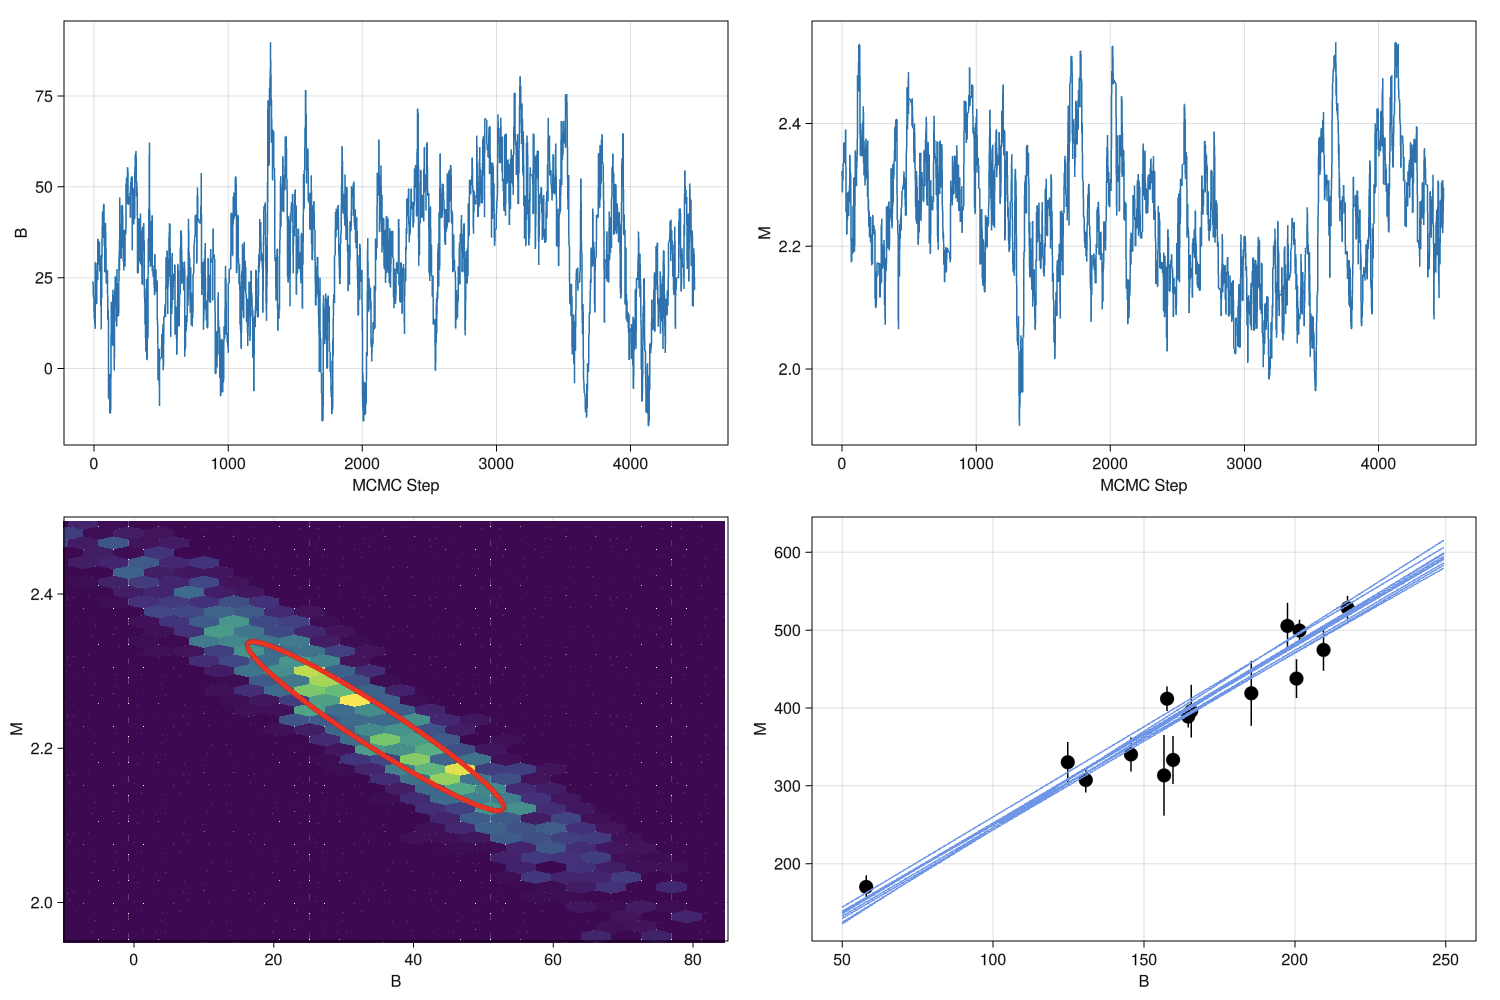
\includegraphics[height=0.8\textheight]{mcmc-results}
\end{frame}


\dfmpage{50}
\dfmpage{53}
\dfmpage{61-62}
\dfmpage{64}
\dfmpage{6}
\dfmpage{70-75}
%\dfmpage{79}

\begin{frame}{Emcee demo}
%\centering
%\scalebox{0.5}{
%}
% DOESNOT GODDAMN WORK
%\multiinclude[<+>][format=png,start=0,end=9,graphics={height=0.8\textheight}]{emcee/emcee}
%\multiinclude[<+->][format=png,start=0,end=9,graphics={height=0.8\textheight}]{emcee/emcee}
\begin{center}
\only<1>{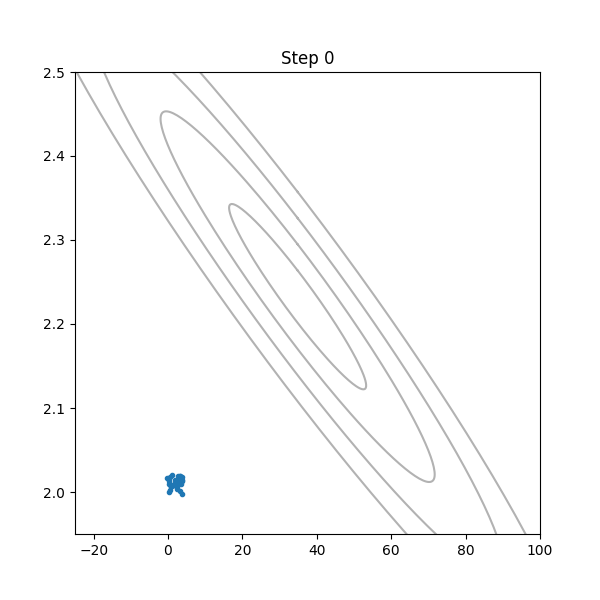
\includegraphics[height=0.8\textheight]{emcee/emcee-0.png}}%
\only<2>{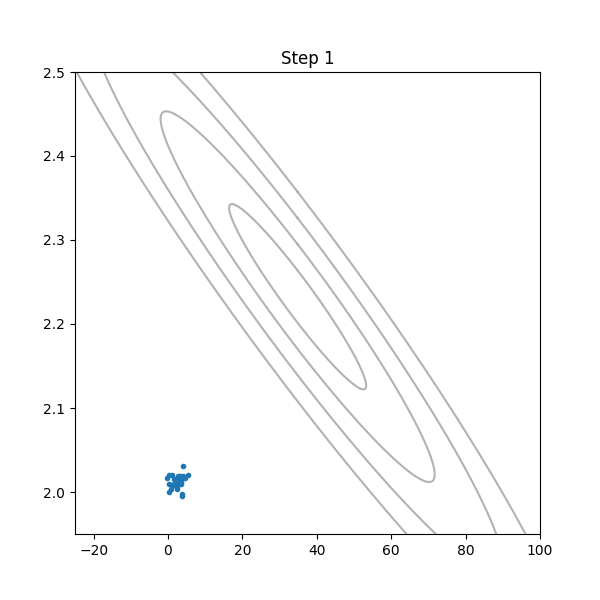
\includegraphics[height=0.8\textheight]{emcee/emcee-1.png}}%
\only<3>{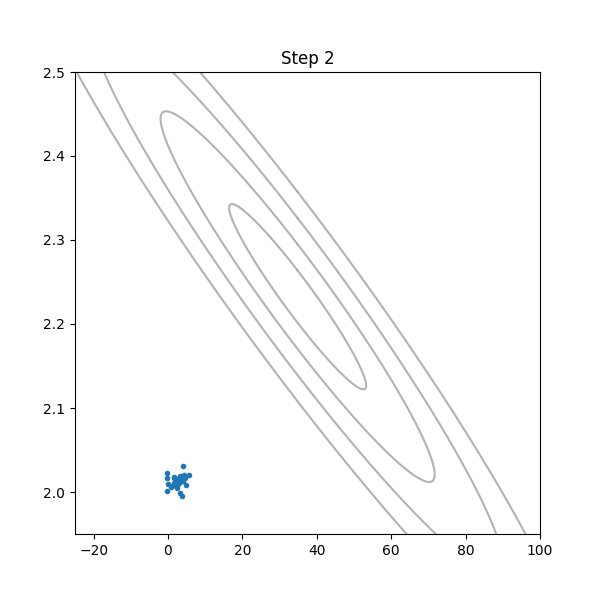
\includegraphics[height=0.8\textheight]{emcee/emcee-2.png}}%
\only<4>{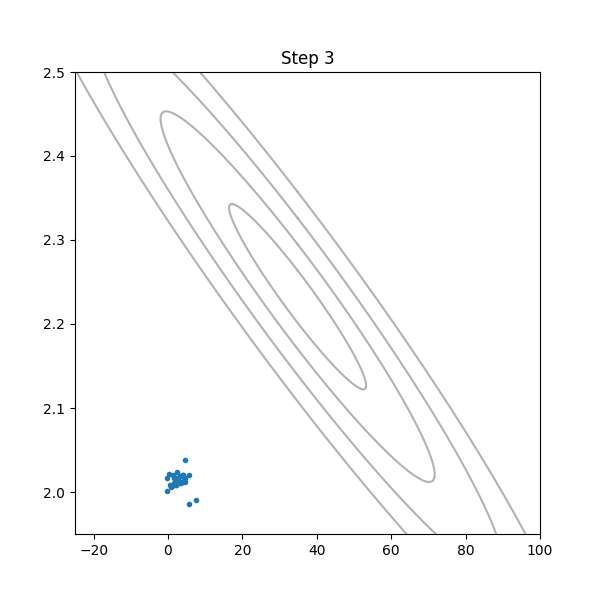
\includegraphics[height=0.8\textheight]{emcee/emcee-3.png}}%
\only<5>{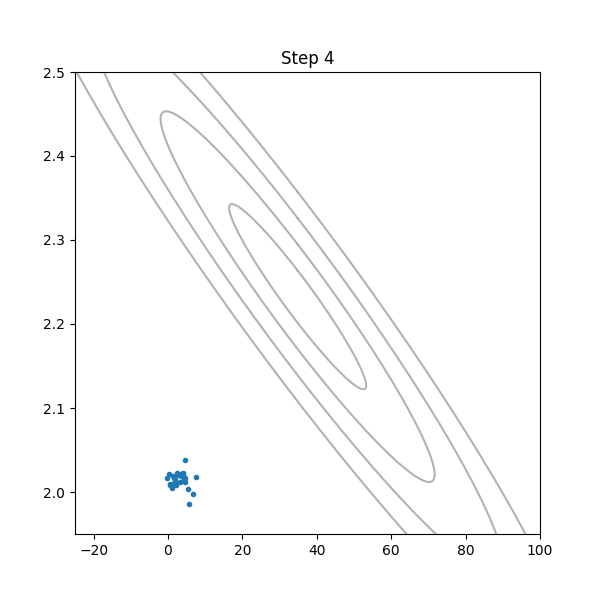
\includegraphics[height=0.8\textheight]{emcee/emcee-4.png}}%
\only<6>{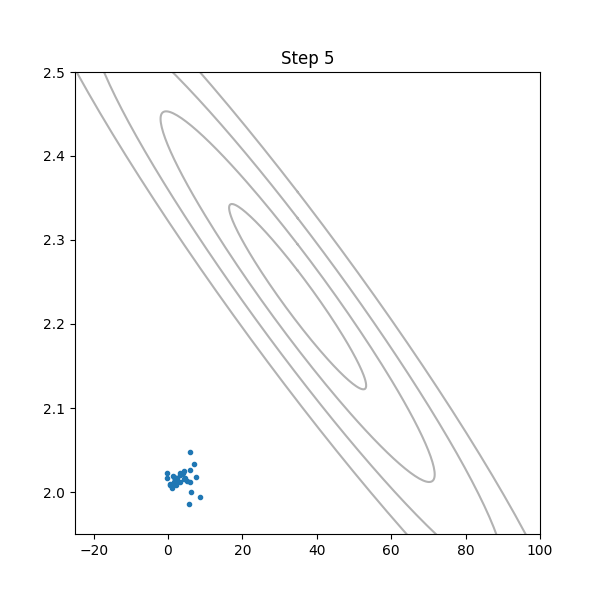
\includegraphics[height=0.8\textheight]{emcee/emcee-5.png}}%
\only<7>{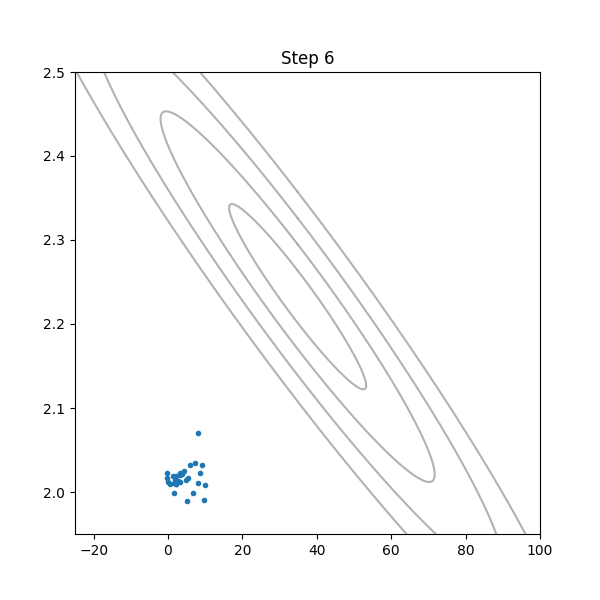
\includegraphics[height=0.8\textheight]{emcee/emcee-6.png}}%
\only<8>{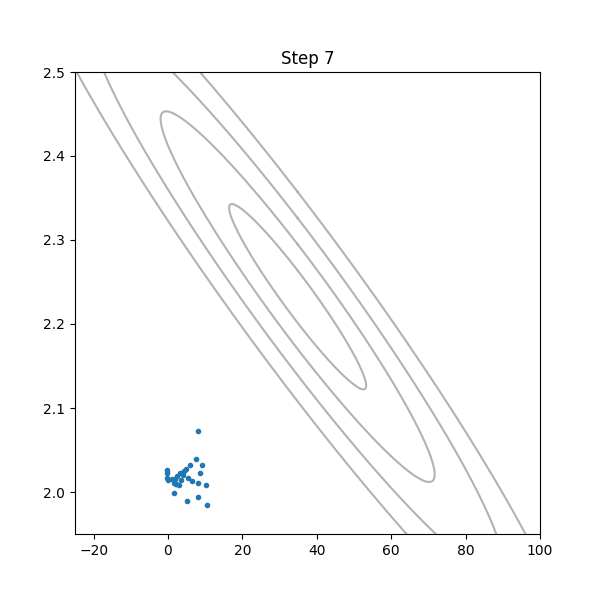
\includegraphics[height=0.8\textheight]{emcee/emcee-7.png}}%
\only<9>{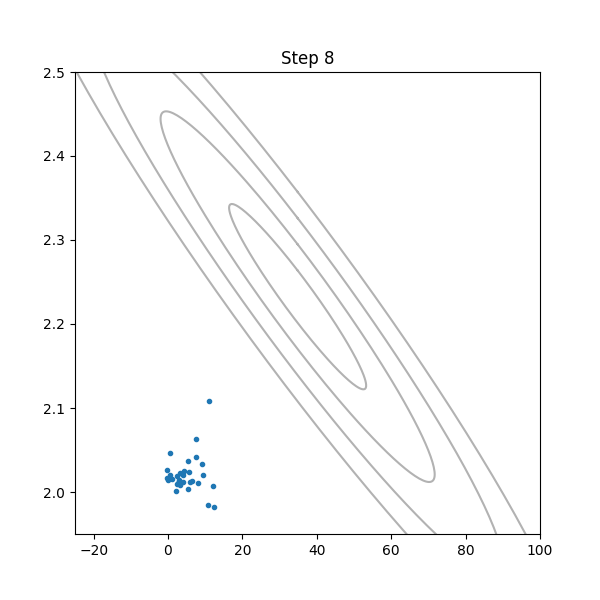
\includegraphics[height=0.8\textheight]{emcee/emcee-8.png}}%
\only<10>{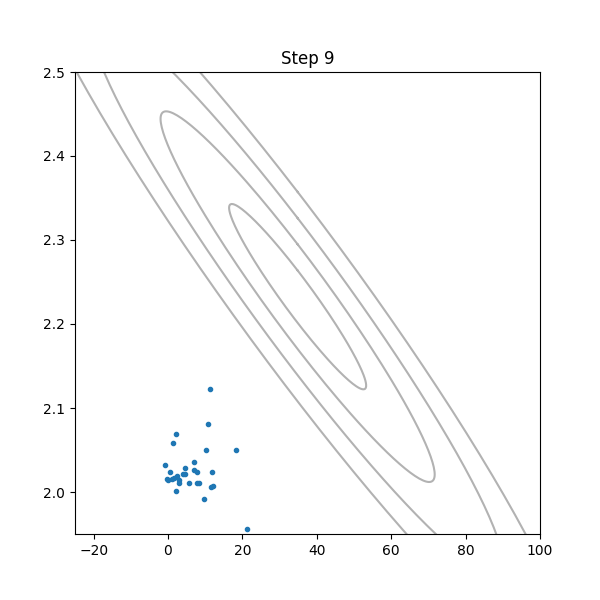
\includegraphics[height=0.8\textheight]{emcee/emcee-9.png}}%
\only<11>{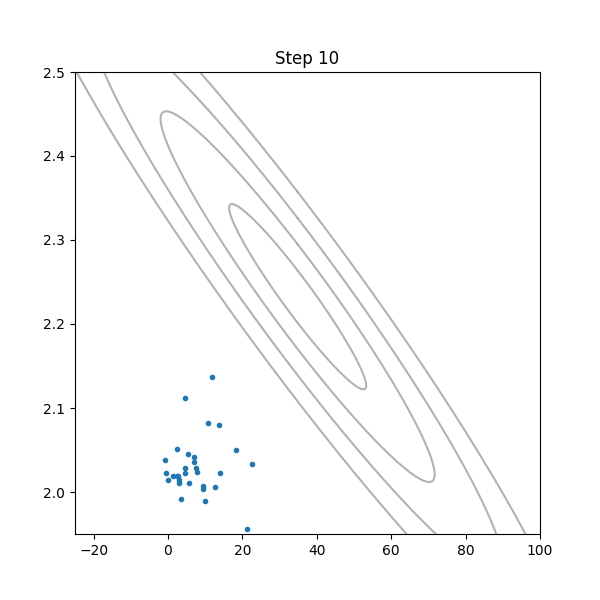
\includegraphics[height=0.8\textheight]{emcee/emcee-10.png}}%
\only<12>{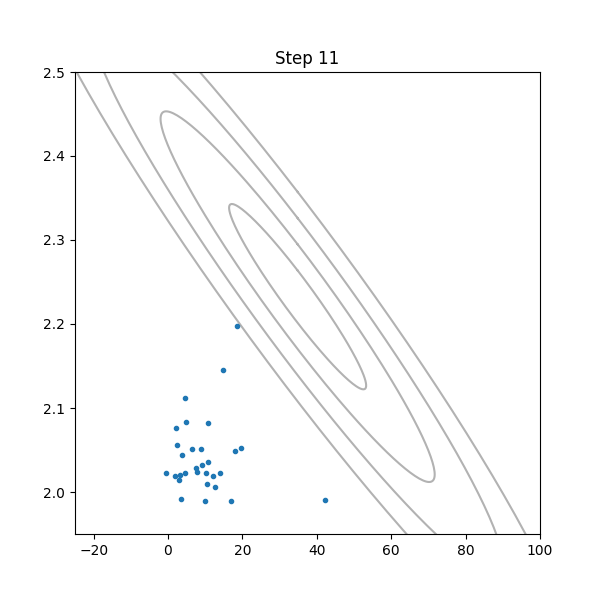
\includegraphics[height=0.8\textheight]{emcee/emcee-11.png}}%
\only<13>{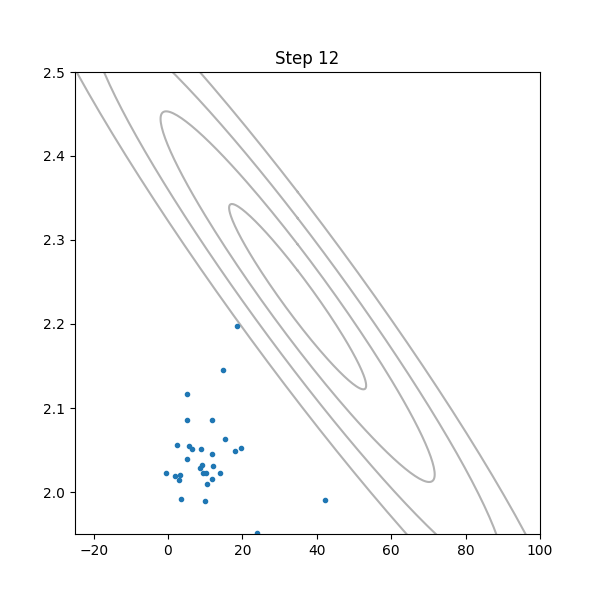
\includegraphics[height=0.8\textheight]{emcee/emcee-12.png}}%
\only<14>{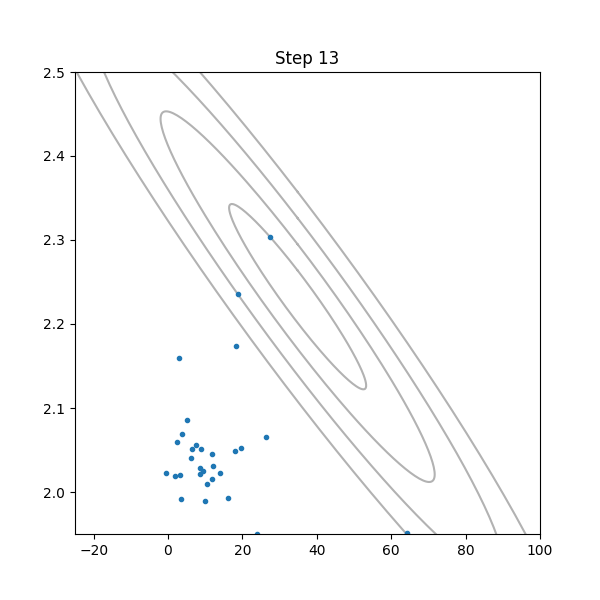
\includegraphics[height=0.8\textheight]{emcee/emcee-13.png}}%
\only<15>{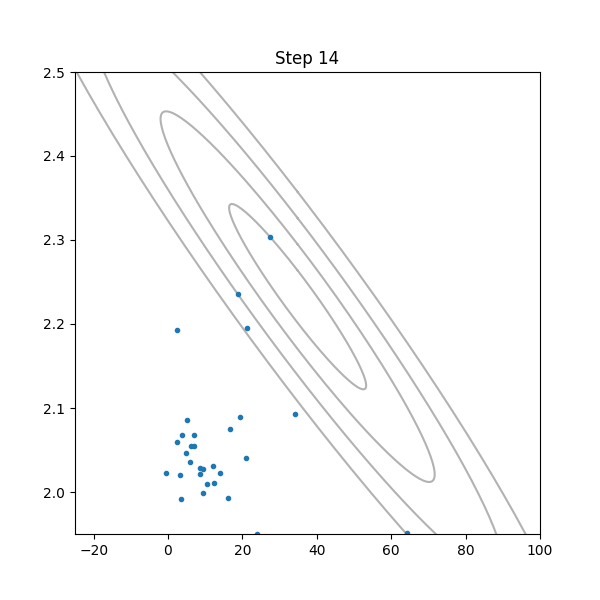
\includegraphics[height=0.8\textheight]{emcee/emcee-14.png}}%
\only<16>{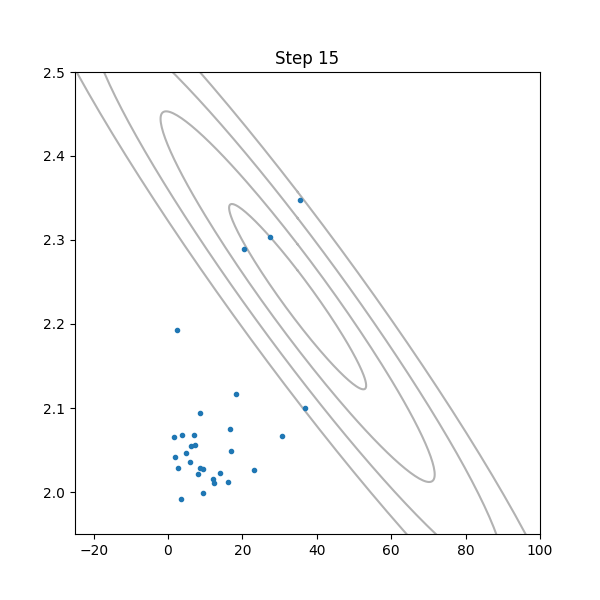
\includegraphics[height=0.8\textheight]{emcee/emcee-15.png}}%
\only<17>{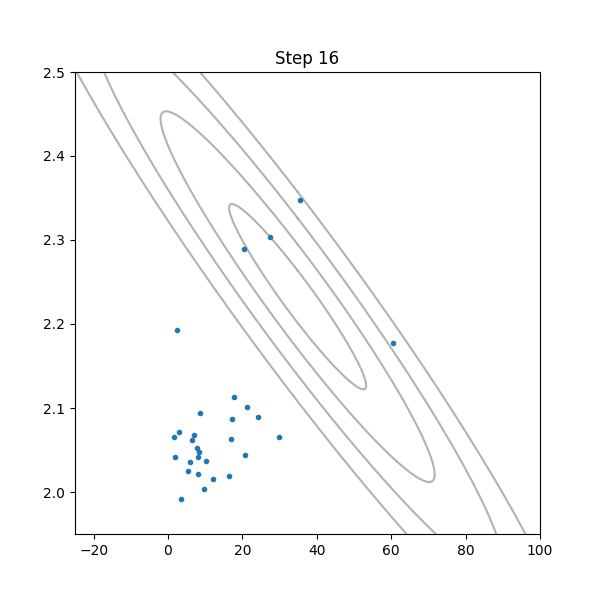
\includegraphics[height=0.8\textheight]{emcee/emcee-16.png}}%
\only<18>{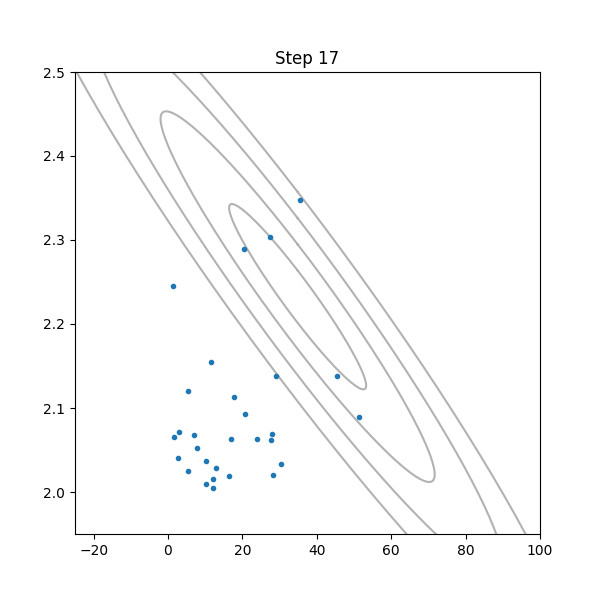
\includegraphics[height=0.8\textheight]{emcee/emcee-17.png}}%
\only<19>{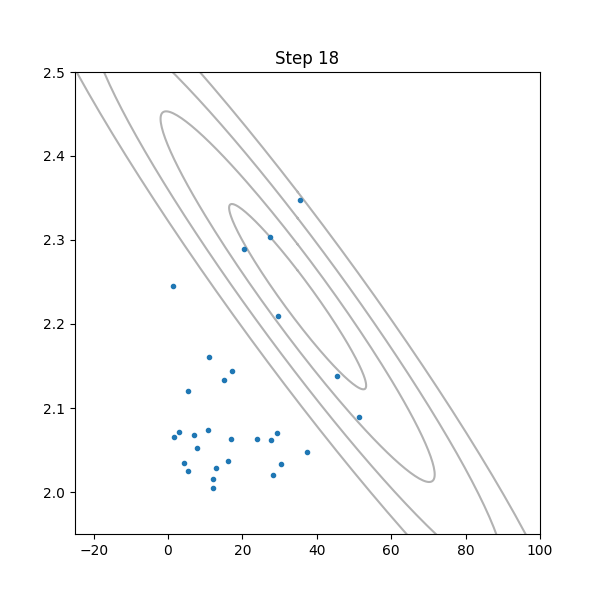
\includegraphics[height=0.8\textheight]{emcee/emcee-18.png}}%
\only<20>{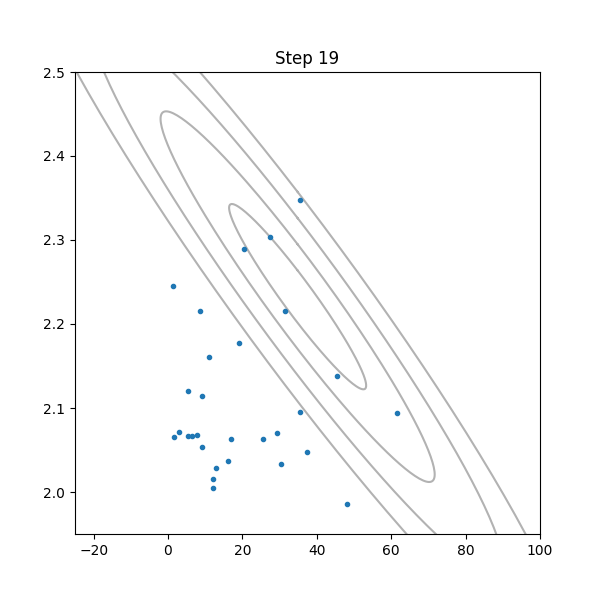
\includegraphics[height=0.8\textheight]{emcee/emcee-19.png}}%
\only<21>{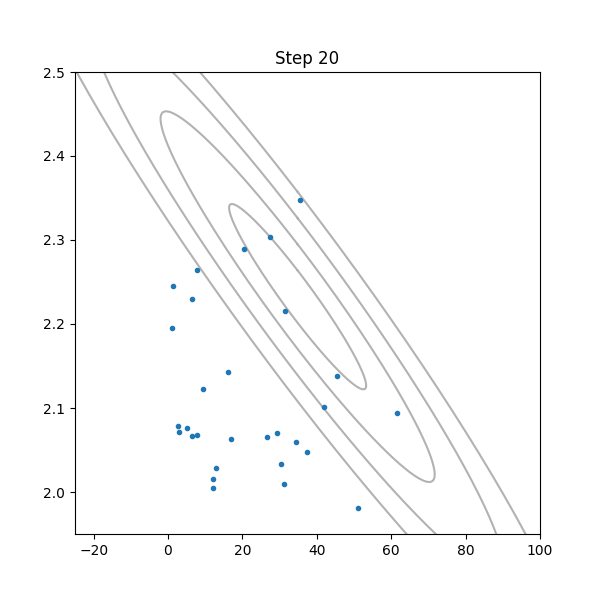
\includegraphics[height=0.8\textheight]{emcee/emcee-20.png}}%
\only<22>{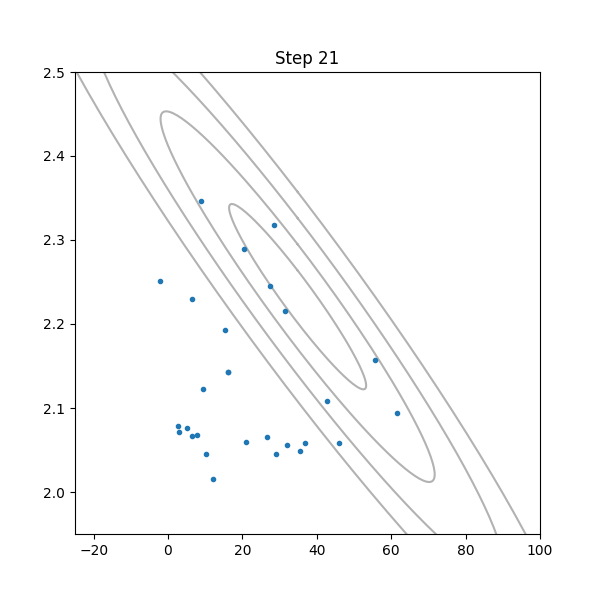
\includegraphics[height=0.8\textheight]{emcee/emcee-21.png}}%
\only<23>{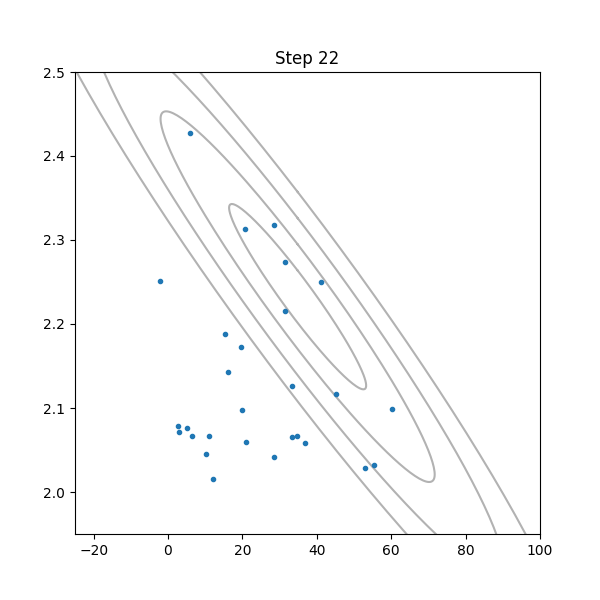
\includegraphics[height=0.8\textheight]{emcee/emcee-22.png}}%
\only<24>{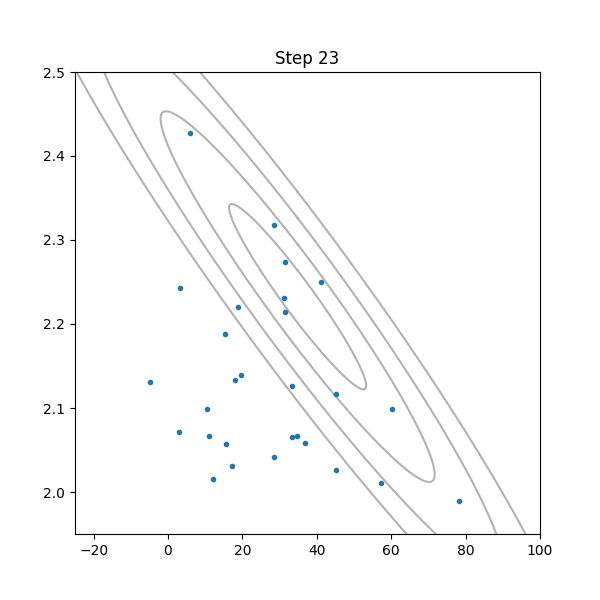
\includegraphics[height=0.8\textheight]{emcee/emcee-23.png}}%
\only<25>{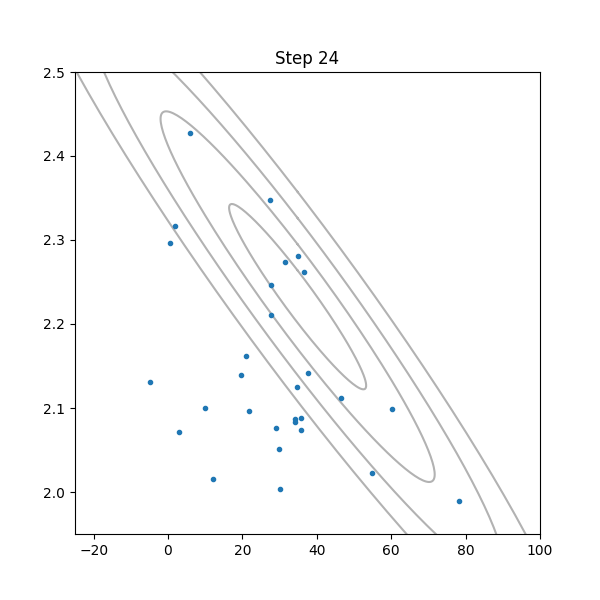
\includegraphics[height=0.8\textheight]{emcee/emcee-24.png}}%
\only<26>{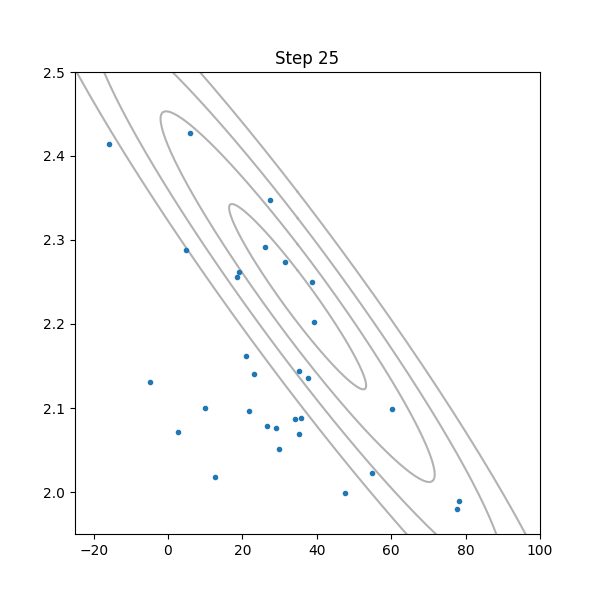
\includegraphics[height=0.8\textheight]{emcee/emcee-25.png}}%
\only<27>{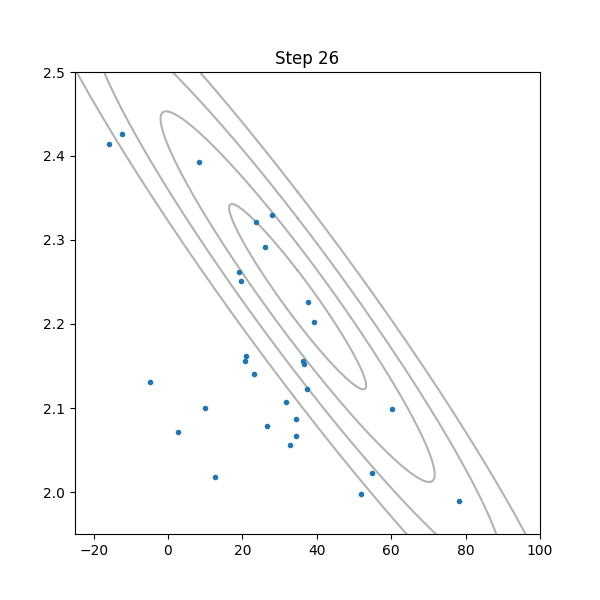
\includegraphics[height=0.8\textheight]{emcee/emcee-26.png}}%
\only<28>{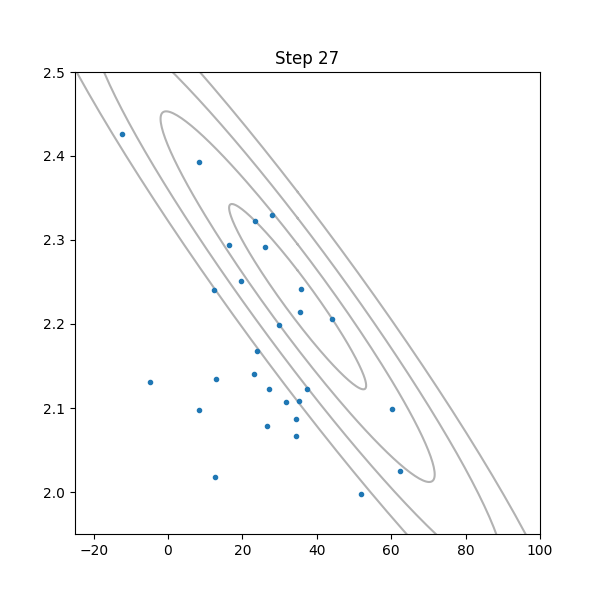
\includegraphics[height=0.8\textheight]{emcee/emcee-27.png}}%
\only<29>{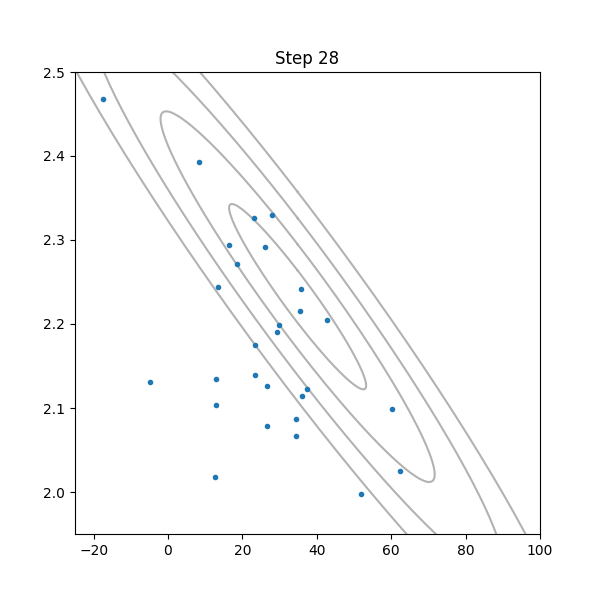
\includegraphics[height=0.8\textheight]{emcee/emcee-28.png}}%
\only<30>{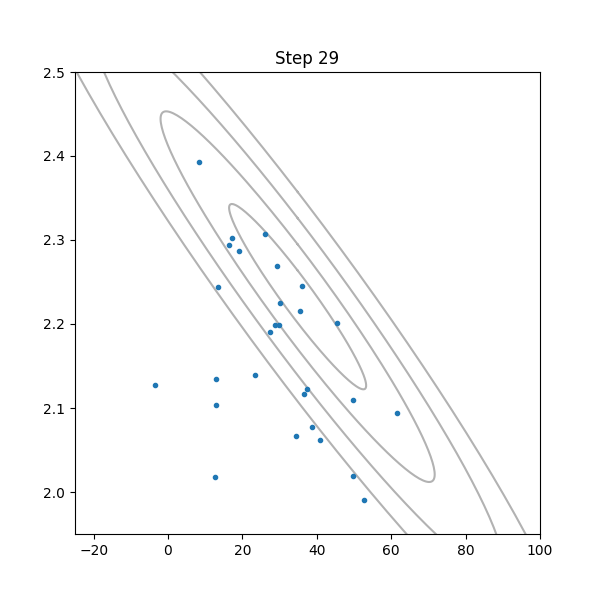
\includegraphics[height=0.8\textheight]{emcee/emcee-29.png}}%
\only<31>{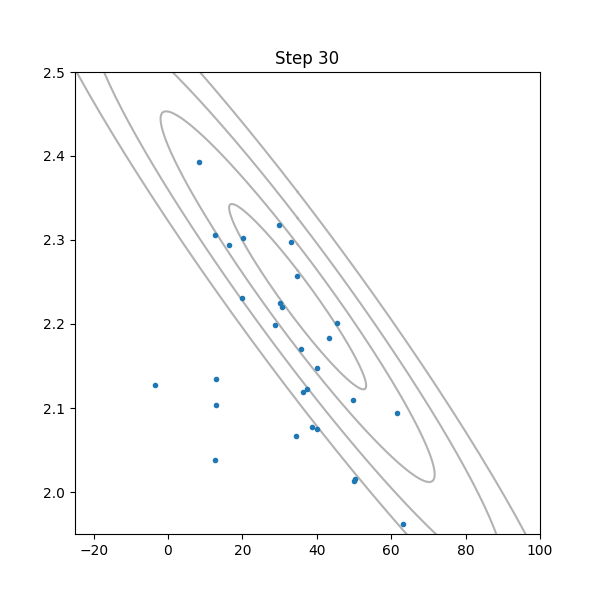
\includegraphics[height=0.8\textheight]{emcee/emcee-30.png}}%
\only<32>{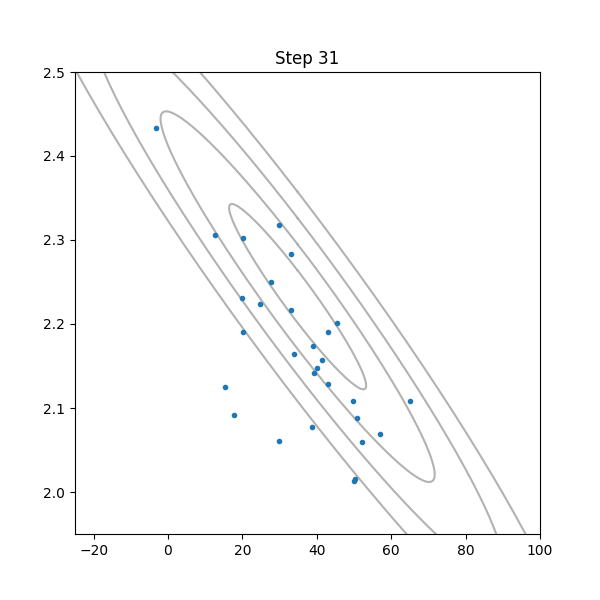
\includegraphics[height=0.8\textheight]{emcee/emcee-31.png}}%
\only<33>{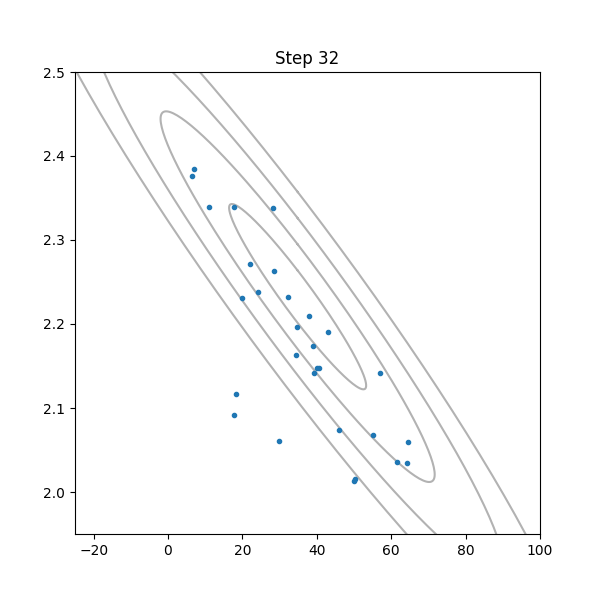
\includegraphics[height=0.8\textheight]{emcee/emcee-32.png}}%
\only<34>{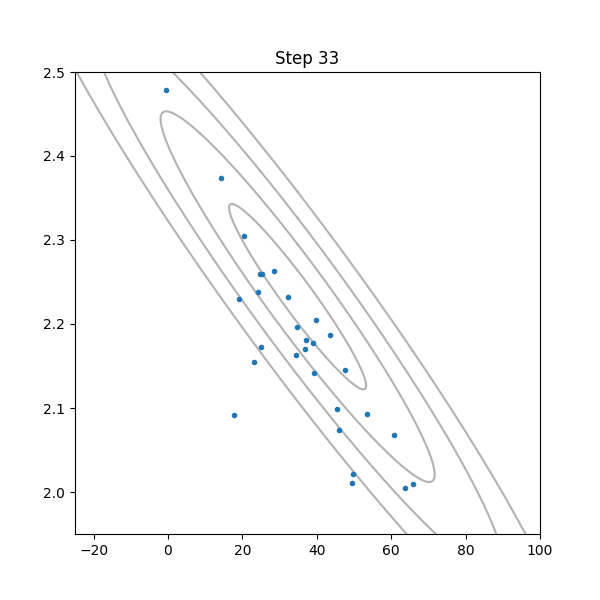
\includegraphics[height=0.8\textheight]{emcee/emcee-33.png}}%
\only<35>{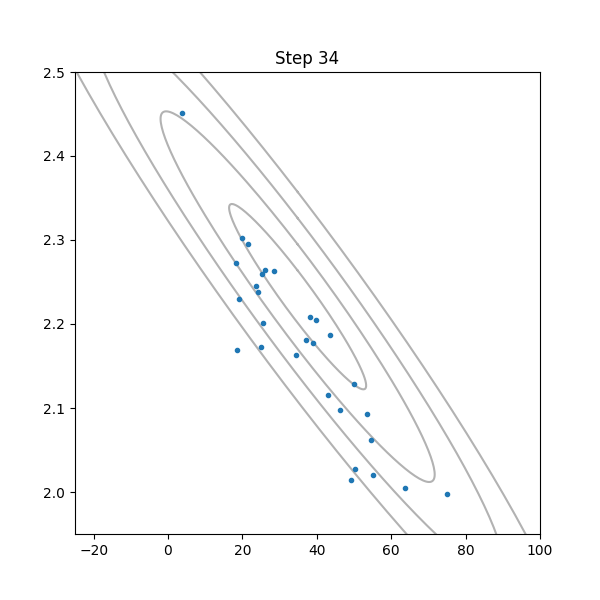
\includegraphics[height=0.8\textheight]{emcee/emcee-34.png}}%
\only<36>{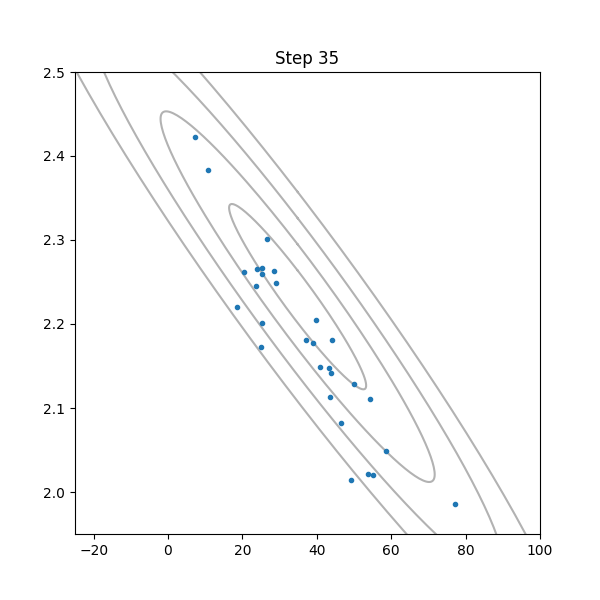
\includegraphics[height=0.8\textheight]{emcee/emcee-35.png}}%
\only<37>{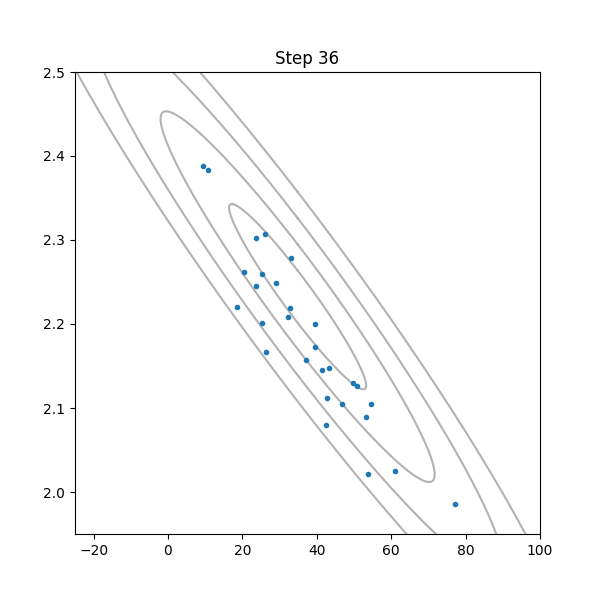
\includegraphics[height=0.8\textheight]{emcee/emcee-36.png}}%
\only<38>{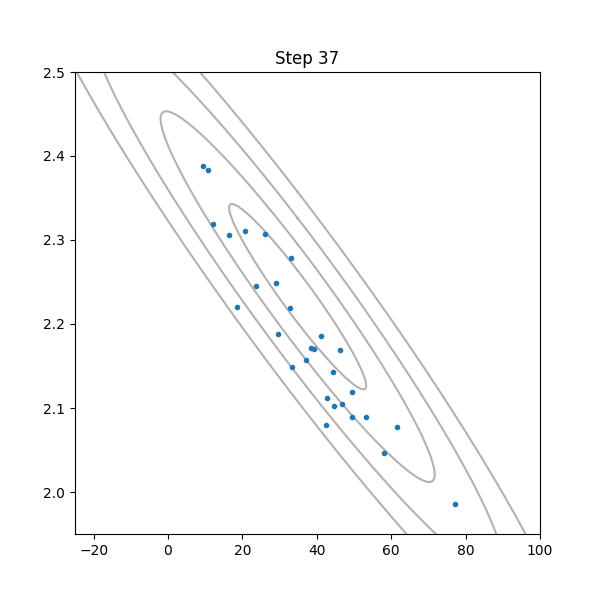
\includegraphics[height=0.8\textheight]{emcee/emcee-37.png}}%
\only<39>{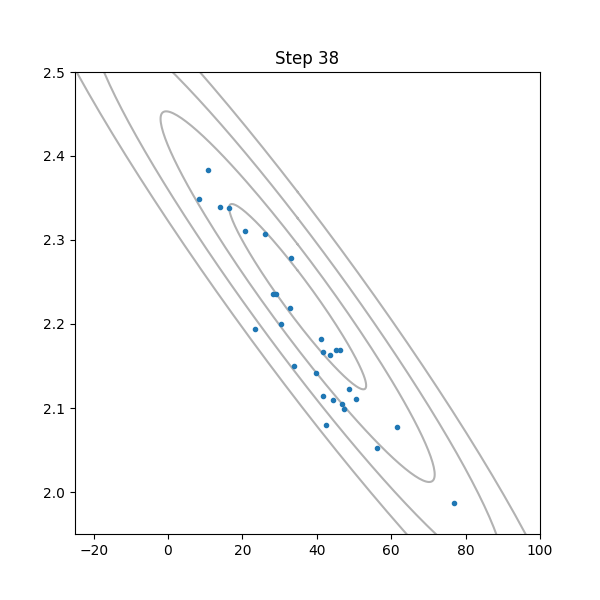
\includegraphics[height=0.8\textheight]{emcee/emcee-38.png}}%
\only<40>{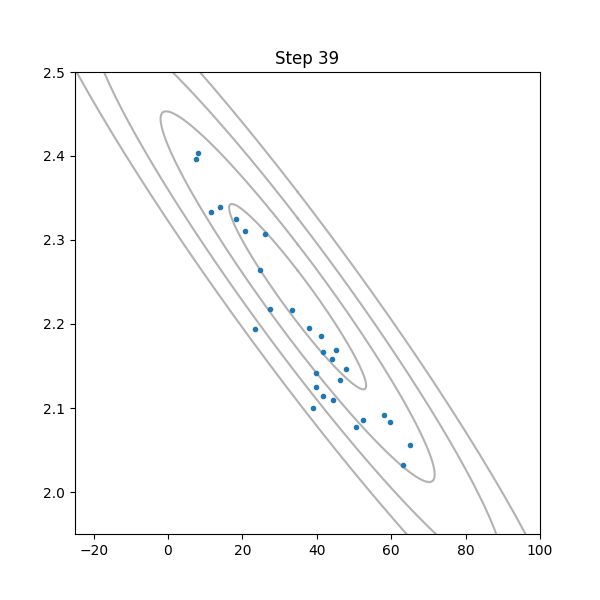
\includegraphics[height=0.8\textheight]{emcee/emcee-39.png}}%
\end{center}
%\multiinclude[format=png,start=0,end=39,height=0.8\textheight]{emcee/emcee}
%\multiinclude[format=png,start=0,end=9,height=0.8\textheight]{emcee/emcee-B}
%\includegraphics[height=0.8\textheight]{emcee/emcee-00}
\end{frame}

\begin{frame}{Emcee demo}
\begin{center}
\only<1>{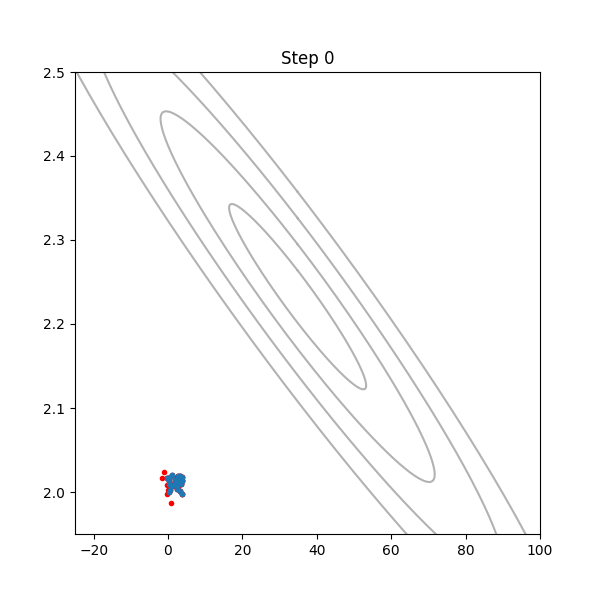
\includegraphics[height=0.8\textheight]{emcee/emcee-B-0.png}}%
\only<2>{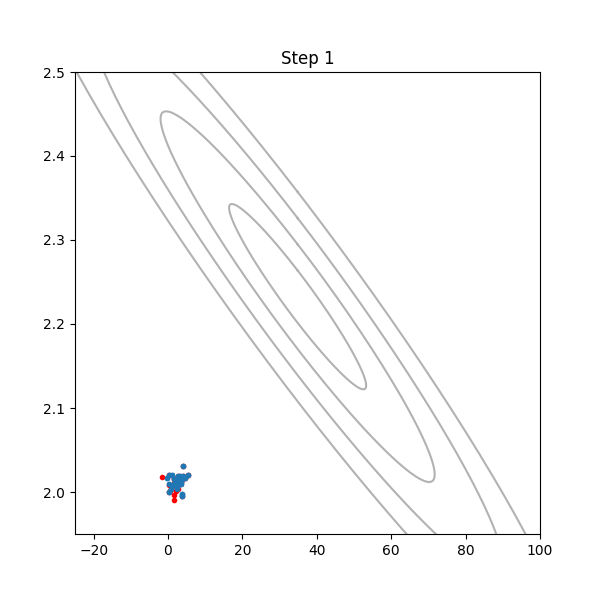
\includegraphics[height=0.8\textheight]{emcee/emcee-B-1.png}}%
\only<3>{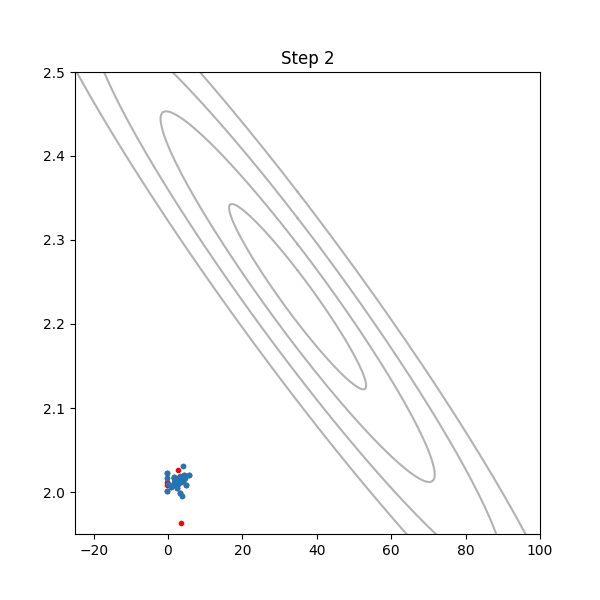
\includegraphics[height=0.8\textheight]{emcee/emcee-B-2.png}}%
\only<4>{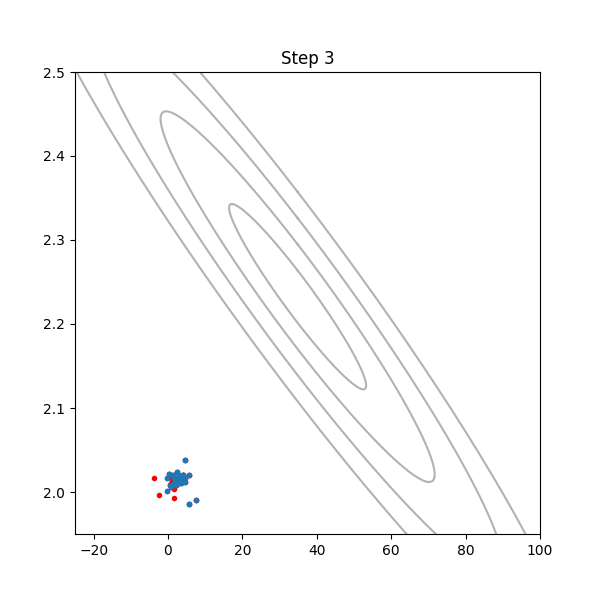
\includegraphics[height=0.8\textheight]{emcee/emcee-B-3.png}}%
\only<5>{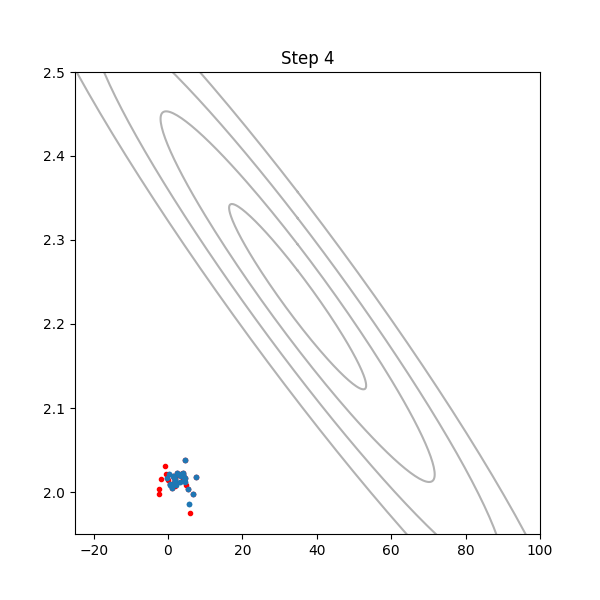
\includegraphics[height=0.8\textheight]{emcee/emcee-B-4.png}}%
\only<6>{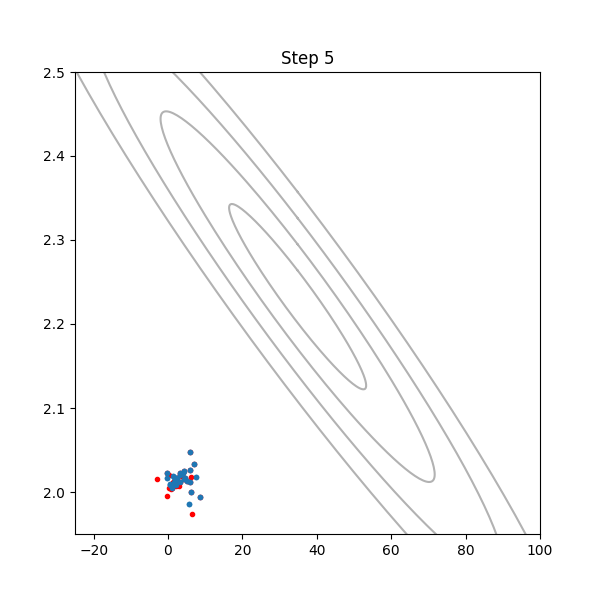
\includegraphics[height=0.8\textheight]{emcee/emcee-B-5.png}}%
\only<7>{\includegraphics[height=0.8\textheight]{emcee/emcee-B-6.png}}%
\only<8>{\includegraphics[height=0.8\textheight]{emcee/emcee-B-7.png}}%
\only<9>{\includegraphics[height=0.8\textheight]{emcee/emcee-B-8.png}}%
\only<10>{\includegraphics[height=0.8\textheight]{emcee/emcee-B-9.png}}%
\end{center}
\end{frame}

%\dfmpage{81}
\dfmpage{106-111}

\begin{frame}{Nested Sampling}
\begin{itemize}
\item An alternative to MCMC (and emcee)
\item (Originally built for integrating the \emph{evidence})
\item Idea: successively resample points, demanding they be above a minimum likelihood level
\item Think of slowly raising the water level to find terrain contours
\end{itemize}
\end{frame}

\jrppage{12-32}
\jrppage{37}

%\begin{frame}{Dynamic Nested Sampling}
%  \includegraphics[height=0.6\textheight]{dynesty-1}
%\end{frame}
\begin{frame}{Dynamic Nested Sampling}
  \includegraphics[height=0.6\textheight]{dynesty-2}
\end{frame}

\begin{frame}{Dynamic Nested Sampling}
%\centering
%\movie[showcontrols,once]{\includegraphics[width=0.4\textwidth]{gal4-01}}{gal4.mov}
%\movie[showcontrols,once]{dynesty logo}{dynesty.gif}
%\animategraphics[loop,width=0.6\textheight]{10}{dynesty-}{0}{79}
%  \includemovie[height=0.6\textheight]{dynesty.gif}
\niceurl{https://dynesty.readthedocs.io/en/stable/}

\niceurl{https://chi-feng.github.io/mcmc-demo/app.html}
\end{frame}


%%%%%%%%%%%%%%%%%%%%%%%%%%%%%%%%%%%%%%




\end{document}

